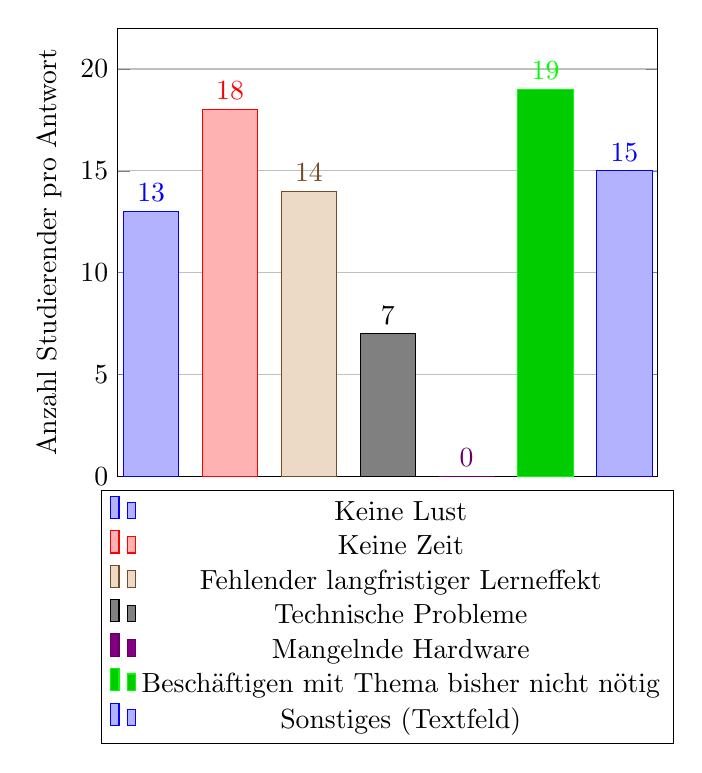
\begin{tikzpicture}
    \begin{axis}[
    	x tick label style={
    		/pgf/number format/1000 sep=},
    	ylabel=Anzahl Studierender pro Antwort,
    	enlarge x limits=2,
        ymax=22,
        ymin=0,
    	legend style={at={(0.5,-0.03)},
        anchor=north,legend columns=1},
        ybar,
        bar width=20pt,
        xticklabels={},
        xtick=\empty,
        nodes near coords,
        grid=major,
    ]
    \addplot coordinates {(1,13)};
    \addplot coordinates {(2,18)};
    \addplot coordinates {(3,14)};
    \addplot coordinates {(4,7)};
    \addplot coordinates {(5,0)};
    \addplot coordinates {(6,19)};
    \addplot coordinates {(7,15)};
    
    \legend{Keine Lust, Keine Zeit, Fehlender langfristiger Lerneffekt, Technische Probleme, Mangelnde Hardware, Beschäftigen mit Thema bisher nicht nötig, Sonstiges (Textfeld)}
    \end{axis}
\end{tikzpicture}